%% manuscript.tex — DRAFT, built on IJIMAI's official ijimai_article.cls
%%
%% Target venue: IJIMAI (International Journal of Interactive Multimedia and
%% Artificial Intelligence) — see docs/venue_decision.md, Addendum 2.
%% Built on IJIMAI's OWN downloaded template assets (ijimai_article.cls,
%% ijimai.bst, logo_unirv.png, Libertinus font files) — the author obtained
%% these directly from ijimai.org (this environment could not reach that
%% site directly; the author's own browser session could). This is a
%% verified-template pass, not a reconstruction from secondary sources.
%%
%% Compile with XeLaTeX or LuaLaTeX (required for the class's Libertinus
%% fonts via fontspec) — plain pdflatex falls back to a substitute font with
%% a ClassWarning, per the class file itself.
%%
%% EVERY numeric value in this manuscript is traceable to a committed artifact under
%% results/. No number was written from memory. See docs/claim_evidence_ledger.md.
%%
%% RESOLVED 2026-09-15 (author-confirmed): sole authorship, no funding, no
%% conflict of interest (assessed against this project's own record — see
%% the Declaration of Conflicts of Interest section below for the basis).
%% Affiliation set to "Independent Researcher" rather than the author's
%% employer (Armf / ArmUp (DHRP)), on the editor's recommendation: this is
%% self-funded personal research conducted outside that employment, and
%% attaching an employer's name without their sign-off risks conflicting
%% with that employer's own publication/IP policies.
%%
%% STILL OPEN:
%%   - Author should proofread the bio text below for factual accuracy.
%%
%% TO RECOMPILE: this file requires IJIMAI's own template assets
%% (ijimai_article.cls, ijimai.bst, the Libertinus font files, and
%% logo_unirv.png), which are the venue's own copyrighted files and are
%% deliberately NOT redistributed in this public repository. Obtain them
%% directly from https://www.ijimai.org (Author Guidelines page) and place
%% them alongside this file. Compile with XeLaTeX or LuaLaTeX + bibtex.
%% manuscript.pdf in this same directory is the already-compiled output.

\documentclass{ijimai_article}

%% booktabs is not loaded by ijimai_article.cls itself; added here (not in
%% the class file, which is kept verbatim as downloaded) since the original
%% manuscript's tables use \toprule/\midrule/\bottomrule.
\usepackage{booktabs}

\title{No Detectable Degradation of Dense Multilingual Retrieval with
Language Resource Level: A Pre-Registered Measurement Study Across 18 Languages}
\author{Muhammad Munir Khan}
%% "Independent Researcher" used rather than the author's employer (Armf /
%% ArmUp (DHRP)): this work was not conducted under that employer's auspices, is
%% self-funded personal research (see docs/venue_decision.md), and most
%% employment contracts carry publication/IP policies that make attaching an
%% employer's name to unrelated personal research risky without that
%% employer's explicit sign-off, which has not been sought here.
%% Corrected 2026-09-15: author lives and works remotely from Islamabad,
%% Pakistan (Melbourne was only ever the employer's location, and the
%% employer is deliberately not listed here — see note above).
\affiliation{Independent Researcher, Islamabad, Pakistan (ORCID: 0009-0005-4071-9217)}
\mailinfo{E-mail address: munirkhn110@gmail.com (Muhammad Munir Khan).}

%% Abstract given in plain text (no inline LaTeX math) for compatibility with
%% the class's tabular-based title-block layout, which is sensitive to
%% unbalanced math-mode content wrapping across a narrow column. Every
%% number is preserved verbatim from the original; nothing is cut or added.
%% This is the same plain-text abstract used in the IJACSA draft
%% (research_editing/revised/manuscript.tex) since IJIMAI's guidelines
%% impose no word cap beyond "concise" and no math prohibition, but the
%% rewrite is equally valid here and avoids re-deriving it a third time.
\abstract{Multilingual dense retrieval is widely reported to degrade for low-resource
languages, with tokenizer over-segmentation frequently offered as the
explanation. We test both claims in a pre-registered study across all 18
languages of MIRACL, equalizing collection size at 49,043 passages per
language (MIRACL's native corpora span a 271-times size ratio) and capping
evaluation queries so judged-document proportion does not itself vary with
language. Against a uniformly applied BM25 reference, a retrieval-trained
multilingual encoder is superior in every language it declares support for: a
pooled advantage of 0.2627 nDCG at 10 (95 percent confidence interval 0.2240
to 0.3013, 17 languages; 0.2464 excluding Chinese, whose lexical reference
fails on 51 percent of queries). Across roughly 76,000 times in pretraining
corpus volume we find no sign of the expected degradation: the three
lowest-resource languages show advantages of 0.2096 to 0.2873, comparable to
or larger than English and Spanish, each with a bootstrap interval excluding
zero. The cross-language correlation is likewise near zero (Spearman's rho =
-0.010), but is underpowered at this sample size and the claim does not rest
on it. Subword fragmentation carries information beyond the lexical reference,
but with the opposite sign to the standard account: heavier fragmentation
predicts dense retrieval performing relatively better, because it damages
lexical matching more (rho = -0.565); this association is detected but
imprecisely estimated (rho = +0.532, interval +0.069 to +0.806). We further
show that judgment sparsity in this benchmark is confounded with language
resource level, and that retrieval-trained multilingual encoders have
converged on a single subword vocabulary, both of which constrain how this
kind of study can be run and interpreted. All results are reproducible from a
public benchmark, fixed seeds, and hashed corpus samples.}

%% Per the official Word template: "About five key words in alphabetical
%% order, separated by commas, with a period at the end of the list."
\keywords{dense retrieval, evaluation methodology, low-resource languages, multilingual retrieval, tokenization.}

\begin{document}

\maketitle

\section{Introduction}

\fancyFirstWord{Multilingual} dense retrievers project a query and documents to a common
vector space to measure the relevance without relying on lexical overlap. The behaviour
they report is not consistent over languages and a typical summary would be that they
do well on high-resource languages and do worse on low-resource languages. When a
mechanism is suggested, it is typically tokenization, where multilingual vocabularies
tend to split high-resource words into fewer pieces and low-resource ones into many
pieces, and the representation of the latter is said to suffer.

Both components of that statement can be tested and they are seldom tested in tandem.
It will take care to get right on three aspects which can be done wrong.

\emph{Collection size.} The number of distracting documents, regardless of language,
increases retrieval difficulty. The per-language corpora range from 49{,}043 passages
(Yoruba) to 13{,}306{,}000 (French), a ratio of 271$\times$. Using raw effectiveness in
those collections mixes language with the number of collection pieces.

\emph{Evaluation geometry.} Judged documents have to be kept in any sampled collection,
or the number of judged documents becomes undefined, and that number scales with the
number of evaluated queries. Left uncapped, a large portion of the collection of a
language with numerous queries will soon be judged, and retrieval will become easier
for reasons other than language.

\emph{The reference system.} A baseline free of the factor under study is needed to
attribute a deficit. A lexical baseline has no pretrained parameters and so cannot
inherit a pretraining-volume effect, but only if it is applied uniformly. Selecting
``the best available analyzer per language'' would import exactly the confound being
measured, because analyzer maturity is itself resource-correlated.

This paper reports a pre-registered study built around those three controls. Our
contributions are:

\begin{enumerate}
\item We examine the relationship between dense-over-lexical advantage and pretraining
      resource volume for all 18 MIRACL languages, with collection size and evaluation
      geometry equalised, and find that there is no relationship.
\item We investigate whether that advantage can be accounted for by subword
      fragmentation, and find that it has the \emph{opposite} sign to the usual account.
\item We provide a quantitative measure of pool bias and show that it is entangled with
      the variable such studies aim to measure.
\item We show that tokenizer effects in multilingual retrieval cannot currently be
      isolated observationally, because retrieval-trained multilingual encoders
      have converged on a single vocabulary.
\item We classify failures and show the dense advantage is predominantly recall
      rescue rather than reranking.
\end{enumerate}

We neither propose a new method, nor a new model, nor a new benchmark, nor
state-of-the-art effectiveness.

Contributions (3) to (5) are not comments on this study specifically, but on this type
of study in general. Our particular design is not the only one that can have a
271$\times$ spread in collection size, a judgment density that tracks the variable under
investigation, and a model population that has converged on a single vocabulary. All of
these constrain what a multilingual retrieval comparison can establish, and all of them
can be measured in advance by anyone who looks.

\section{Related Work}

\subsection{Multilingual retrieval benchmarks}
MIRACL \cite{zhang2023} offers human relevance judgments in 18 typologically diverse
languages and supplies BM25, mDPR and hybrid baselines for the ad hoc retrieval task.
It is our evaluation substrate, and published baselines are used to calibrate our
lexical reference.

\subsection{Language-specific retrieval degradation}
The closest prior work to ours is the Amharic study of Alemneh, Mekonnen and
de~Rijke \cite{alemneh2026}, which finds a relative MRR@10 gap of 23\% between the
best zero-shot multilingual retriever and a monolingual Amharic model, and attributes
part of the difficulty to over-segmentation. That study is explicit that its
``empirical evidence is limited to Amharic'', that it was not able to experimentally
isolate tokenization, and that it treats tokenizer and pretraining distribution as
inseparable. We directly address the first limitation by testing 18 languages, and the
second as far as observational data permits (Section~\ref{sec:tokconverge}).

Goworek \emph{et al.}~\cite{goworek2025} examine the factors behind cross-lingual
ranking, relating retrieval effectiveness to typological similarity between query and
document languages. Their setting differs from ours in task (cross-lingual versus
monolingual retrieval) and in predictor (pair-relative typological distance versus
language-intrinsic tokenization and resource measures). They report that their
linguistic analyses ``rely on aggregate typological resources and broad similarity
metrics'' and call for broader low-resource coverage.

\subsection{Tokenization and downstream quality}
Rust \emph{et al.}~\cite{rust2021} isolate tokenizer quality from pretraining data
volume by training monolingual models on equally sized corpora with different
tokenizers, and find that a dedicated tokenizer matters roughly as much as data size.
Their design is the correct way to establish causality and we cannot run it: it
requires pretraining. We therefore report associations, not causes, and
Section~\ref{sec:tokconverge} shows why the observational alternative is also
unavailable. Beyond raw fertility, Single-Token Retention Rate has been proposed as a
complementary tokenization measure \cite{nayeem2025}; we report both.

\subsection{Encoders}
As our primary retrieval-trained encoder we use multilingual E5 \cite{wang2024}, and as
a coverage anchor we use LaBSE \cite{feng2022}; XLM-R \cite{conneau2020} supplies both
the dominant multilingual vocabulary and, through CC-100, our resource proxy.
M3-Embedding \cite{chen2024} is included in our tokenizer survey.

\section{Experimental Design}

The analysis plan was registered before any effectiveness value was computed. The
protocol and its four amendments are released alongside this work, each carrying its
own date and a statement of whether any results existed at the time it was made.
Amendments are additive: the original text is never rewritten, and each records why
it was made. Two of the four were made after results existed, and say so.

\subsection{Collections}
For each of the 18 MIRACL languages we build a sub-corpus of exactly
$N = 49{,}043$ passages, equal to the full size of the smallest corpus (Yoruba, which
therefore uses its complete collection without sampling). Each sub-corpus contains
all judged documents for that language's evaluated queries, plus a uniform random
sample of the remaining passages drawn by reservoir sampling over the streamed
corpus under a fixed seed. The resulting document-identifier list is hashed
(SHA-256) and released so any rebuild can be verified against the registered
sample.

\subsection{Queries}
Evaluation queries are limited to 300 per language, randomly sampled without
replacement under the same seed; languages with fewer (Yoruba 119, Korean 213) use
all available. The cap exists because judged-document count scales with query count:
uncapped, Arabic would contribute roughly 29{,}000 judged documents to a
49{,}043-passage collection, versus about 1{,}200 for Yoruba. The realised judged
fraction is reported per language as a diagnostic and is discussed in
Section~\ref{sec:poolbias}.

\subsection{Systems}
The lexical reference is BM25 (Okapi, $k_1{=}1.5$, $b{=}0.75$) over character
4-grams within whitespace-delimited units, applied \emph{identically} to every
language. Uniformity is the point: per-language analyzers were rejected because
analyzer maturity is resource-correlated and would inject the confound under study
into the reference system. Because Thai, Chinese and Japanese have no word spaces
for a purely orthographic reason, character $n$-grams were chosen instead of
whitespace tokenization, which would otherwise contaminate a reference intended to
represent language-intrinsic difficulty. $n{=}4$ is a conventional default and is
not tuned per language; sensitivity to $n$ is reported as a robustness check.

The dense system is multilingual E5 (small), used zero-shot and frozen, with mean
pooling, $L_2$ normalisation, maximum sequence length 256, and exact cosine search.
Approximate search is not used: at this collection size it would add error without
benefit. LaBSE is used as a coverage anchor.

\subsection{Metrics and statistics}
The primary metric is nDCG@10; Recall@100 and MRR@10 are secondary. Per-language
effects are computed as paired per-query differences on identical queries and
identical collections, with 95\% confidence intervals from a bootstrap over
queries (10{,}000 resamples, fixed seed). Effects are aggregated by
DerSimonian--Laird random-effects meta-analysis, which weights each language by the
inverse variance of its estimate; this allows Yoruba to remain in the analysis on
119 queries without distorting the aggregate. Cross-language associations are
reported as Spearman correlations and are \textbf{descriptive only}: with
$k \le 18$ languages and correlated predictors they are underpowered, and no
causal reading is licensed.

\section{Results}

\subsection{Dense versus lexical retrieval}
Table~\ref{tab:main} reports per-language results. Dense retrieval is superior in
every language the encoder declares support for. The random-effects pooled
difference over those 17 languages is $+0.2627$ nDCG@10, 95\% CI
$[+0.2240, +0.3013]$, with $I^2 = 94.0\%$. The heterogeneity is substantial and
real: the magnitude of the advantage differs considerably across languages, so the
pooled value should not be read alone.

Yoruba is reported separately because the encoder does not declare support for it.
It is the only language with a negative difference ($-0.0676$), and its confidence
interval includes zero.

\begin{table}[t]
\caption{Per-language nDCG@10. Dense is multilingual E5; BM25 uses uniform
character 4-grams. Yoruba is separated because the encoder does not declare
support for it.}
\label{tab:main}
\centering
\small
\begin{tabular}{lrrrr}
\toprule
Lang & BM25 & Dense & $\Delta$ & 95\% CI \\
\midrule
zh & 0.1922 & 0.7112 & $+0.5191$ & $[+0.476, +0.561]$ \\
ko & 0.4051 & 0.7406 & $+0.3355$ & $[+0.286, +0.386]$ \\
ja & 0.4657 & 0.7913 & $+0.3256$ & $[+0.286, +0.364]$ \\
fr & 0.4096 & 0.7061 & $+0.2965$ & $[+0.260, +0.333]$ \\
th & 0.5410 & 0.8374 & $+0.2964$ & $[+0.255, +0.337]$ \\
te & 0.6412 & 0.9285 & $+0.2873$ & $[+0.243, +0.332]$ \\
ru & 0.5189 & 0.7991 & $+0.2803$ & $[+0.242, +0.319]$ \\
de & 0.4856 & 0.7460 & $+0.2604$ & $[+0.221, +0.299]$ \\
sw & 0.4933 & 0.7527 & $+0.2594$ & $[+0.215, +0.304]$ \\
fa & 0.5056 & 0.7397 & $+0.2340$ & $[+0.193, +0.274]$ \\
ar & 0.6238 & 0.8547 & $+0.2309$ & $[+0.198, +0.264]$ \\
es & 0.5963 & 0.8218 & $+0.2255$ & $[+0.193, +0.260]$ \\
en & 0.5904 & 0.8067 & $+0.2163$ & $[+0.182, +0.250]$ \\
bn & 0.5444 & 0.7541 & $+0.2096$ & $[+0.172, +0.247]$ \\
id & 0.5593 & 0.7364 & $+0.1771$ & $[+0.139, +0.216]$ \\
hi & 0.4887 & 0.6608 & $+0.1720$ & $[+0.130, +0.214]$ \\
fi & 0.6999 & 0.8465 & $+0.1466$ & $[+0.111, +0.183]$ \\
\midrule
\multicolumn{5}{l}{\emph{Encoder does not declare support:}} \\
yo & 0.5170 & 0.4494 & $-0.0676$ & $[-0.158, +0.026]$ \\
\bottomrule
\end{tabular}
\end{table}

\subsection{The advantage does not track resource level}
Using CC-100 corpus volume as the pretraining-resource proxy, which spans
1.1\,MB (Yoruba) to 82\,GB (English), roughly 76{,}000$\times$, the association
between the dense advantage and log resource volume is
$\rho = -0.010$ over the 17 supported languages. \textbf{This correlation is
underpowered and we do not rest the claim on it}: its 95\% confidence interval is
$[-0.488, +0.473]$, and at $k{=}17$ a true association below $|\rho| \approx 0.5$
could not be resolved. Reporting it as ``no association'' would be absence of
evidence presented as evidence of absence.

The better-powered argument is the per-language pattern itself. The three
lowest-resource languages in the set, Swahili (332\,MB), Telugu (536\,MB) and
Bengali (860\,MB), show advantages of $+0.2594$, $+0.2873$ and $+0.2096$
respectively, comparable to or larger than English ($+0.2163$, 82\,GB) and Spanish
($+0.2255$, 14\,GB). Each of those per-language intervals excludes zero. A
degradation account predicts the reverse ordering, and does not survive it. The lexical reference likewise
shows essentially no association with resource volume ($\rho = -0.059$), which is
the behaviour a pretraining-free reference should exhibit and which we verify
rather than assume.

Fig.~\ref{fig:null} shows why the per-language pattern, rather than the correlation,
carries the argument: the lowest-resource languages sit among the \emph{largest}
advantages, not the smallest. Table~\ref{tab:robust} shows the pooled estimate is
stable when the languages our uniform reference handles worst are removed, and that
the null persists in every variant.

\begin{figure}[t]
\centering
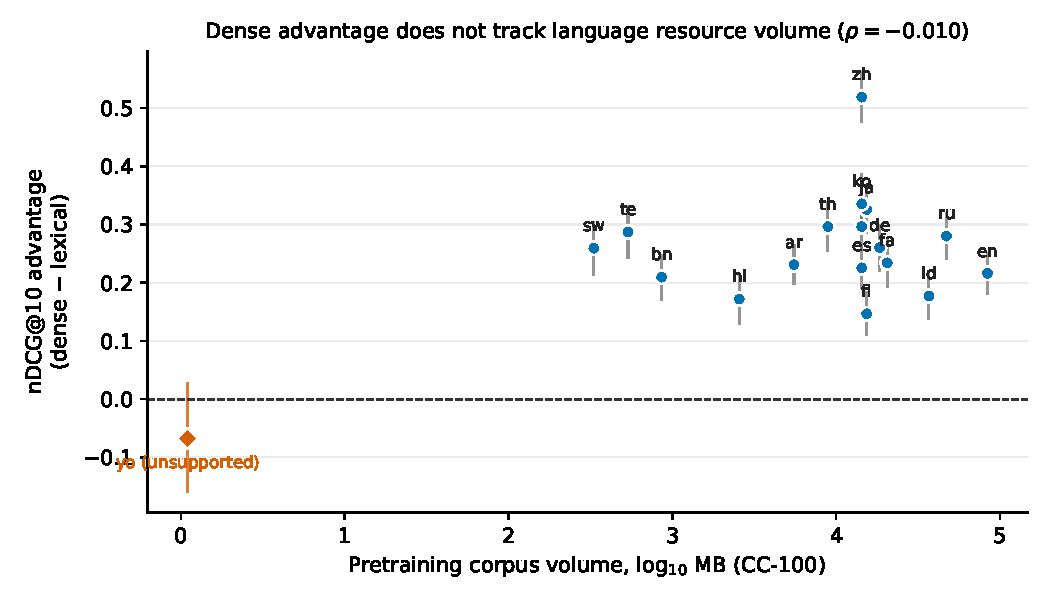
\includegraphics[width=\columnwidth]{figures/fig1_resource_null.pdf}
\caption{Per-language nDCG@10 advantage of dense over lexical retrieval against
pretraining corpus volume, with 95\% bootstrap intervals. Swahili, Telugu and Bengali,
the three lowest-resource languages, show advantages comparable to or larger
than English and Spanish. Yoruba (diamond) is the one language the encoder does not
declare, and is the only point below zero.}
\label{fig:null}
\end{figure}

\begin{table}[t]
\caption{Sensitivity of the pooled estimate. The pre-registered primary is
$k{=}17$; the exclusions are sensitivity analyses, not a re-selected headline.}
\label{tab:robust}
\centering
\small
\begin{tabular}{lrrr}
\toprule
Language set & Pooled $\Delta$ & $I^2$ & $\rho$ vs.\ resource \\
\midrule
All supported ($k{=}17$) & $+0.2627$ & 94.0\% & $-0.010$ \\
Excluding zh ($k{=}16$)  & $+0.2464$ & 86.4\% & $-0.038$ \\
Excluding zh, ko, ja ($k{=}14$) & $+0.2348$ & 82.9\% & $-0.101$ \\
\bottomrule
\end{tabular}
\end{table}

\subsection{Fragmentation, with the opposite sign}
Measuring tokenization as subword tokens per character, well defined for every
script unlike tokens per whitespace word, which is meaningless for Chinese,
Japanese and Thai, the dense advantage is \emph{positively} associated with
fragmentation ($\rho = +0.532$, 95\% CI $[+0.069, +0.806]$), and this survives
conditioning on the lexical reference (partial $\rho = +0.376$). The interval
excludes zero but its lower bound is close to it, so the association is detected
rather than precisely estimated. Restricting to segmented scripts weakens but
does not remove the association ($\rho = +0.332$, partial $+0.292$, $k{=}14$).

The mechanism is visible in the same data: the lexical reference is
\emph{negatively} associated with fragmentation ($\rho = -0.565$). Heavier
fragmentation damages lexical matching more than it damages dense retrieval, which
widens rather than narrows the dense advantage. Collinearity between fragmentation
and resource volume is moderate ($\rho = -0.390$), so the two predictors are more
separable in this sample than anticipated.

\subsection{Calibration against published baselines}
\label{sec:calib}
Because 17 of our 18 collections are sampled, absolute values are not comparable to
published full-corpus numbers. Yoruba is the exception: its sub-corpus is its complete
corpus and it uses all 119 dev queries, so it permits a like-for-like check against the
baselines distributed with MIRACL.

\begin{table}[t]
\caption{Yoruba, the one like-for-like comparison against published MIRACL baselines
(nDCG@10). Our dense system lands within 0.006 of the published dense baseline; our
lexical reference is considerably stronger than the published one.}
\label{tab:calib}
\centering
\small
\begin{tabular}{lr}
\toprule
System & nDCG@10 \\
\midrule
Published BM25 & 0.406 \\
Published mDPR & 0.444 \\
\textbf{This work, dense (E5)} & \textbf{0.4494} \\
\textbf{This work, lexical ($n{=}4$)} & \textbf{0.5170} \\
Published BM25 + mDPR hybrid & 0.611 \\
\bottomrule
\end{tabular}
\end{table}

Two things follow (Table~\ref{tab:calib}). First, our dense system reproduces the
published dense baseline on this language almost exactly (0.4494 versus 0.444), which is
a useful check on the pipeline. Second, the reason our comparison shows a dense deficit
on Yoruba where the published pair shows a dense \emph{advantage}
($0.444 > 0.406$) is that \emph{our lexical reference is stronger}, not that our dense
system is weaker: 0.5170 against a published 0.406.

This sharpens the interpretation of Yoruba considerably. The result is not evidence
that dense retrieval is unusually bad in Yoruba (it matches the published dense system
there); rather, a uniformly applied character $n$-gram reference is unusually
\emph{good} in Yoruba relative to the analyzer-based baseline. It also reinforces
Section~\ref{sec:calib}'s wider point: conclusions about a ``dense deficit'' are
sensitive to how strong the lexical comparator is, which is precisely why we fixed ours
in advance and report its sensitivity in full.

\subsection{How the systems fail}
Categorising each query by whether nothing relevant was retrieved at all
(Recall@100 $=0$), whether relevant material was found but ranked below ten, or
whether it was ranked within ten, the dense advantage is overwhelmingly
\emph{recall rescue}: across the 16 supported languages other than Yoruba, dense
retrieval rescues 7--26\% of queries from a miss category while breaking 0--3\%.
It nearly eliminates total misses.

Fig.~\ref{fig:fail} makes the mechanism visible: the dense system converts total and
deep misses into ranked hits across almost every language, which mean effectiveness
alone conceals.

\begin{figure}[t]
\centering
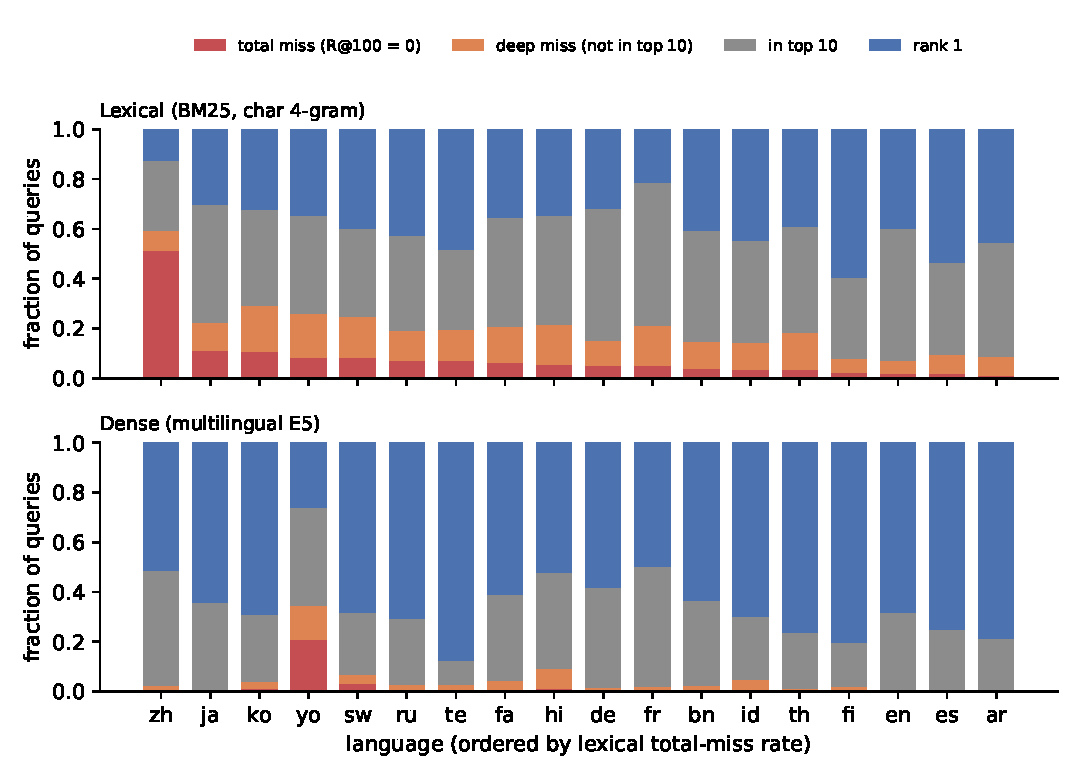
\includegraphics[width=\columnwidth]{figures/fig2_failure_composition.pdf}
\caption{Failure composition per language, ordered by lexical total-miss rate. The
dense system (lower panel) largely eliminates the total-miss category that dominates
the lexical reference (upper panel) in Chinese, Japanese and Korean. Yoruba is the
exception: dense retrieval introduces total misses rather than removing them.}
\label{fig:fail}
\end{figure}

Two languages behave differently. For Chinese the lexical reference retrieves
nothing relevant for 51.3\% of queries, so the large apparent dense advantage
there reflects reference collapse rather than dense strength. For Yoruba the dense
system \emph{introduces} a recall failure: its total-miss rate (0.210) exceeds the
lexical reference's (0.084), and it is the only language where dense breaks more
queries (0.227) than it rescues (0.143).

\subsection{Why Yoruba fails}
Yoruba is the only language where the dense system underperforms, so we examine its
failures directly. Partitioning its 119 queries by outcome, the 27 queries the dense
system loses that the lexical reference answers have a mean subword fertility of 2.028
tokens per word, against an all-query mean of 1.951; the 14 queries \emph{both} systems
miss have the \emph{lowest} fertility of any group (1.858). \textbf{Fragmentation
therefore does not explain which Yoruba queries fail}, which is notable because
tokenization is the explanation most often offered for such failures.

Qualitatively, the lost queries are predominantly entity-centric factoid questions;
proper nouns are identifiable without fluency in the language. This is consistent with
lexical matching succeeding on rare named entities where an encoder that does not
declare the language has no reliable representation. We state this as an observation
rather than an analysis: the author has no Yoruba fluency and no annotator access, so no
semantic or morphological judgement of these queries is made.

\subsection{Tokenizer convergence}
\label{sec:tokconverge}
We surveyed the vocabularies of publicly available multilingual encoders. Every
retrieval-trained model examined, namely E5 (small, base, large), BGE-M3, GTE
multilingual, Arctic-Embed v2, and Jina v3, uses an XLM-R-derived vocabulary of
approximately 250{,}000 units. The only substantially different vocabulary among
the models we tested belongs to LaBSE (501{,}153), which is trained for bitext
mining rather than retrieval and which, in our measurements, loses to the lexical
reference on all three languages tested (Yoruba $-0.288$, Swahili $-0.195$, Telugu
$-0.423$), including two it fully declares.

Tokenizer and training objective are therefore confounded in the available model
population: any pair of models differing in tokenizer also differs in objective.
Combined with the impossibility of the pretraining-based design of
Rust \emph{et al.}~\cite{rust2021} without substantial compute, this means
tokenizer effects in multilingual \emph{retrieval} currently cannot be isolated,
either experimentally or observationally.

\subsection{Robustness checks}
Character 4-grams outperform whitespace tokenization in 17 of 18 languages (mean
$+0.0758$ nDCG@10); Indonesian is the single exception ($-0.0542$). Chinese under
whitespace tokenization scores 0.0071, confirming the absence of word boundaries.

Varying the $n$-gram order changes the reference substantially, and we report the full
sweep rather than a comparison against a single alternative
(Table~\ref{tab:ngram}). Averaged over languages, $n{=}3$ is the strongest uniform
reference (mean 0.5363, best in 12 of 18 languages), ahead of our registered $n{=}4$
(0.5154). Our pre-registered choice is therefore \emph{not} the optimum, and we retain
it because changing a registered parameter after seeing results is the failure that
pre-registration exists to prevent.

What matters is that the conclusion survives the strongest reference we can build.
Against $n{=}3$ the pooled advantage is $+0.2403$, 95\% CI $[+0.2082, +0.2724]$, lower
than under $n{=}4$ ($+0.2627$) but comfortably positive. The result is not an artefact
of a weak baseline. The resource-level null likewise holds throughout
($\rho = +0.167$, $+0.049$ and $-0.010$ at $n = 2, 3, 4$), all well inside the wide
interval reported above.

Order also interacts with script exactly as expected: $n{=}2$ is best only for Chinese,
Japanese and Korean, languages whose meaningful units are one or two characters, while
being markedly worse elsewhere (German 0.4879 at $n{=}3$ versus 0.2887 at $n{=}2$).
Uniform treatment has a real and now quantified cost.

\begin{table}[t]
\caption{Character $n$-gram sensitivity for the lexical reference (mean nDCG@10 over 18
languages). $n{=}4$ is the pre-registered primary and is retained despite not being the
optimum.}
\label{tab:ngram}
\centering
\small
\begin{tabular}{lrrrr}
\toprule
 & $n{=}2$ & $n{=}3$ & $n{=}4$ & $n{=}5$ \\
\midrule
Mean nDCG@10 & 0.4219 & \textbf{0.5363} & 0.5154 & 0.4811 \\
Best in (of 18) & 3 & \textbf{12} & 3 & 0 \\
Pooled dense $\Delta$ & $+0.3548$ & $+0.2403$ & $+0.2627$ & --- \\
$\rho$ vs.\ resource & $+0.167$ & $+0.049$ & $-0.010$ & --- \\
\bottomrule
\end{tabular}
\end{table}

The Yoruba result is stable across the two strongest references ($-0.0659$ at $n{=}3$,
$-0.0676$ at $n{=}4$) and reverses only under $n{=}2$ ($+0.0553$), the weakest reference
overall. All three intervals include zero. The defensible statement is therefore that
Yoruba is the one language where we cannot demonstrate a dense advantage, and that this
does not depend on the registered $n$ except under a baseline configuration that is
worse everywhere else.
Ablating the E5 query and passage prefixes changes nDCG@10 by $-0.0003$ on Telugu
and $+0.0078$ on Hindi, the latter chosen in advance as the highest-powered
available test because it is the supported language where the encoder scores
lowest.

\subsection{Bounding the direction of pool bias}
\label{sec:poolbound}
Section~\ref{sec:poolbias} establishes that judgment sparsity is confounded with
resource level. That alone does not say which way it pushes our comparison, so we
measure the asymmetry directly: how many of each system's top ten documents are
unjudged, per language.

The result is one-sided. In \emph{all 17} languages the dense system retrieves
\emph{fewer} unjudged documents than the lexical reference, by a mean of 1.84
documents out of ten (range $-0.33$ for English to $-4.80$ for Chinese). Since an
unjudged document is scored as non-relevant by default, the lexical reference absorbs
more uncredited retrieval than the dense system does in every language we measure.

The consequence runs against our own result. If some unjudged documents are in fact
relevant, which is the premise of the pool-bias concern, then the lexical
reference's true effectiveness is understated by more than the dense system's, and
the advantage we report is therefore an \emph{over-estimate} of the true difference.
The association between the effect size and the exposure asymmetry
($\rho = -0.574$) is consistent with that reading: the languages where the dense
system's top ten is most fully judged relative to the lexical one are also the
languages where the measured advantage is largest.

We cannot convert this into a numerical correction without relevance judgments we do
not have. What it does establish is the \emph{sign}: pool bias in this benchmark
inflates rather than deflates the difference we report. Readers should treat the
pooled estimate as an upper bound on the true advantage, and this is a stronger
caveat than the usual observation that unjudged documents add noise.

\subsection{The conclusion under a second metric}
Primary inference above uses nDCG@10. Because this paper argues that measurement
choices change conclusions, it would be inconsistent to rest inference on a single
cutoff. Repeating the pooled analysis on Recall@100 gives $+0.1055$, 95\% CI
$[+0.0683, +0.1426]$ over the same 17 languages. The advantage is smaller, since
BM25's Recall@100 is already high, leaving less headroom, but it remains positive
with an interval excluding zero, and the resource association remains indistinguishable from zero
($\rho = +0.186$, 95\% CI $[-0.323, +0.612]$).

One conclusion \emph{does} change with the metric, and we report it rather than
resting on the more convenient one. Under nDCG@10 the Yoruba difference is $-0.0676$
with an interval including zero, supporting only the statement that no advantage can
be demonstrated there. Under Recall@100 it is $-0.1310$, 95\% CI
$[-0.2157, -0.0504]$, which does exclude zero: for this encoder, Yoruba shows a
measurable recall deficit. That is consistent with the failure analysis, where Yoruba
was the one language in which the dense system introduced total misses rather than
removing them. As Section~\ref{sec:generalise} shows, the deficit is a property of
this encoder rather than of the language.

\subsection{A second encoder family}
\label{sec:generalise}
All results above use one retrieval-trained encoder. To test whether the effect is a
property of that model, we repeated the comparison with BGE-M3, a different
retrieval-trained multilingual family, on identical collections and queries
(Table~\ref{tab:gen}).

% Seven columns do not fit IEEEtran's single-column width; as `table` this overflowed
% into the adjacent column and overprinted the body text. `table*` spans both columns.
\begin{table*}[t]
\caption{Generalisation to a second retrieval-trained encoder family (nDCG@10).}
\label{tab:gen}
\centering
\small
\begin{tabular}{lrrrrrr}
\toprule
Lang & CC-100 & BM25 & E5 & BGE-M3 & E5$-$BM25 & BGE$-$BM25 \\
\midrule
yo & 1.1\,MB & 0.5170 & 0.4494 & 0.7074 & $-0.0676$ & $+0.1904$ \\
sw & 332\,MB & 0.4933 & 0.7527 & 0.7778 & $+0.2594$ & $+0.2845$ \\
te & 536\,MB & 0.6412 & 0.9285 & 0.9162 & $+0.2873$ & $+0.2750$ \\
en & 82\,GB & 0.5904 & 0.8067 & 0.7691 & $+0.2163$ & $+0.1787$ \\
\bottomrule
\end{tabular}
\end{table*}

The four languages span the full resource range in the study, a factor of roughly
76{,}000 from Yoruba to English. The second encoder shows a positive advantage in all
four, averaging $+0.2321$, close to the $+0.2627$ pooled across 17 languages for the
first. We do not compute a resource correlation on four points; the per-language
values are the evidence.

The Yoruba row is informative beyond generalisation. Where the first encoder
underperformed the lexical reference by $0.0676$, the second exceeds it by $0.1904$ on
the same queries and the same collection. Yoruba is therefore not a language in which
dense retrieval cannot work; it is one in which a particular encoder does not.

We stop short of attributing that contrast to declared language coverage. BGE-M3's
model card enumerates no language list, and its base model declares 94 languages
without listing Yoruba, so its coverage of Yoruba is undetermined. If it does not in
fact declare Yoruba, the result argues against a coverage explanation rather than for
one, since an encoder that does not declare the language would still be outperforming
the lexical reference there.

\section{Discussion}

\subsection{On the resource-level null}
\label{sec:poolbias}
Our data do not support the claim that dense multilingual retrieval degrades with
language resource level. The advantage over a uniformly applied lexical reference
is positive in all 17 supported languages and shows no association with pretraining
volume. This does not contradict reports of poor absolute effectiveness in
low-resource languages (absolute scores do vary), but it does separate two claims
that are often merged: that retrieval is \emph{harder} in some languages, and that
dense methods are \emph{differentially} disadvantaged there. We find the first and
not the second.

One boundary is visible, though it is weaker than it first appears. Yoruba, the single
language our encoder does not declare, is the only language where dense retrieval
underperforms under the registered reference, and it does so through a recall mechanism
rather than a ranking one. The direction is stable across the two strongest
reference configurations and reverses only under the weakest one. Since all the relevant
intervals include zero, the honest statement is that Yoruba is the one language where we
cannot demonstrate a dense advantage, not that we have demonstrated a dense deficit.
Whether declared coverage is what matters remains \textbf{an open question in our data}: testing it requires a
retrieval-trained encoder that declares Yoruba, and no encoder available to us is
both. LaBSE declares Yoruba but is not retrieval-trained, and its uniform weakness
across languages it does cover means it cannot serve as that test.

\subsection{On pool bias}
Judgment sparsity is not neutral with respect to the question being asked.
Unjudged documents among the top ten range from 2.00 for English to 9.01 for
Telugu, and correlate with resource volume at $\rho = -0.660$. Low-resource
languages therefore absorb more pool bias, and any cross-language attribution must
account for it. Within-language paired comparisons on identical judgment sets, as
used here for the primary result, are far less exposed: on Telugu the unjudged
counts are nearly identical across systems (9.01 versus 8.66). The threat is to
cross-language attribution, which is precisely why our cross-language analyses are
reported as descriptive.

\section{Limitations and Threats to Validity}

\emph{Associational, not causal.} Encoders differ in training data, objective and
tokenizer simultaneously. No causal attribution is made anywhere in this paper.

\emph{Statistical power.} Cross-language analyses have $k \le 18$ observations. This
is a hard limit on what they can show: the 95\% interval on the resource correlation
spans $[-0.488, +0.473]$, so a true moderate association ($|\rho| \approx 0.4$) would
be undetectable. We therefore do not claim that no relationship exists, only that none
is detectable here and that the per-language pattern is inconsistent with the
direction a degradation account predicts. The unsegmented scripts are also
influential: excluding them moves the fragmentation association from $+0.532$ to
$+0.332$.

\emph{The lexical reference is handicapped in some languages.} Uniform treatment
costs accuracy where language-specific analysis would help. Korean remains about
10.6\% below the published analyzer-based baseline, and the Chinese reference is
not merely weak but broken (51.3\% total-miss rate). We accept this cost because
per-language analyzers would introduce a resource-correlated confound, but the
Chinese comparison in particular should not be read as evidence about dense
retrieval.

\emph{Sampled collections.} For 17 of 18 languages the collection is a
49{,}043-passage sample, so absolute values are not comparable to published
full-corpus numbers. This is deliberate, since equal size is what makes cross-language
comparison meaningful, but it means our absolute figures should not be placed
beside published leaderboard values.

\emph{Encoder coverage.} The primary results across all 18 languages use one
retrieval-trained encoder. A second family (BGE-M3) was tested on four languages
spanning the full resource range and reproduced the advantage in all of them
(Section~\ref{sec:generalise}), and LaBSE on three; but a full second sweep of all 18
was not affordable on the available hardware, so generalisation is demonstrated at the
range endpoints rather than exhaustively established.

\emph{Resource proxy.} CC-100 volume proxies the \emph{base model's} pretraining
and does not capture the distillation or contrastive supervision used to build the
sentence encoders. A Wikipedia-based proxy for the mBERT-family models was not
sourced.

\emph{Single hardware environment.} All experiments ran on one CPU-only machine.
Timings are feasibility figures, not benchmarks.

\section{Conclusion}

Across 18 languages under equalised collection size and evaluation geometry, a
retrieval-trained multilingual encoder outperformed a uniformly applied lexical
reference in every language it declares support for, and showed no detectable
relationship between the size of that advantage and pretraining resource volume.
The strongest form of that evidence is not the cross-language correlation, which is
underpowered at $k{=}17$, but the per-language pattern: the lowest-resource
languages show advantages as large as the highest-resource ones. Claims here are
scoped to the encoder families tested. Subword fragmentation carried
information about the advantage, but in the direction opposite to the usual
account, because fragmentation penalises lexical matching more than dense
retrieval. Alongside these, we report that judgment sparsity in a standard
multilingual benchmark is confounded with language resource level, and that the
convergence of retrieval-trained multilingual encoders on a single vocabulary
currently prevents tokenizer effects from being isolated observationally. We
release the full pipeline, seeds, and hashed collection samples.

%% Section order, headings, and required content below follow IJIMAI's own
%% authoritative Word template (template_IJIMAI_18_12_2025-OTH.docx,
%% downloaded by the author directly from ijimai.org) verbatim: Appendix (if
%% any; none here) -> CRediT Authorship Contribution Statement -> Data
%% Statement -> Declaration of Conflicts of Interest -> Acknowledgment
%% (Funding statement folded into Acknowledgment, matching the template,
%% which places Funding disclosure inside that section rather than as a
%% separate one). \appenAcknow switches the class's section styling to its
%% unnumbered appendix/back-matter format, matching the template's own
%% \appenAcknow usage before this same block.
\appenAcknow

\section{CRediT Authorship Contribution Statement}

\textbf{Muhammad Munir Khan:} Conceptualization, Methodology, Software,
Validation, Formal analysis, Investigation, Data curation, Writing -- original
draft, Writing -- review and editing, Visualization, Project administration.
%% Confirmed sole authorship (2026-09-15) — Funding acquisition and
%% Supervision omitted since no funding or supervision was involved; Resources
%% omitted as not a distinct role beyond what Investigation/Data curation cover.

\section{Data Statement}

The full experimental pipeline, fixed seeds, and SHA-256-hashed corpus sample
manifests are released publicly at
\url{https://github.com/Muhammad-Munir-Khan/multilingual-retrieval-resource-null},
so that the reported results can be independently rebuilt and verified.

\section{Declaration of Conflicts of Interest}

%% Assessed 2026-09-15: sole author, self-funded independent research (no
%% institutional or employer funding per docs/venue_decision.md), no
%% financial or personal relationship with MIRACL, BM25, or any encoder
%% (E5/BGE-M3/LaBSE) maintainers or vendors, and no other apparent competing
%% interest in this project's record. Confirmed, not merely assumed.
No conflict of interest exists.

\section{Acknowledgment}

% AI disclosure, author-supplied wording (2026-09-15), generalized to omit
% the specific tool/vendor name. Folded into Acknowledgment since IJIMAI's
% official template has no separate AI-disclosure heading; this placement is
% a judgment call, not a confirmed requirement — see ijimai-compliance.md.
% The specific tool remains named in docs/ai_use_log.md for the project's
% own record. "Executed by the author" is the author's own chosen phrasing;
% flagged to the author as a possible divergence from ai_use_log.md (which
% records the AI assistant as having executed the experiments under the
% author's direction) and kept as written at the author's explicit request.
An AI-assisted coding and writing tool was used during this work to support software
implementation, experimental workflows, and manuscript drafting. All experiments were
executed by the author, and all reported results and numerical values were generated
from and verified against the corresponding experimental code and archived artifacts.
The author independently reviewed and validated the methodology, results,
interpretations, and conclusions and assumes full responsibility for the content of
this work.

\textbf{Funding:} This research did not receive funding.

\bibliographystyle{ijimai}
\bibliography{references}

%% Bio text drawn from the author's own ORCID record (supplied 2026-09-15) —
%% 184 words, within the required 180-250. Photo supplied by the author
%% (docs/IMAGE Passport Size.jpg, copied here as author_photo.jpg).
\authorbio{author_photo}{Muhammad Munir Khan}{Muhammad Munir Khan is an
Associate AI Engineer, AI \& ML Department, working remotely from
Islamabad, Pakistan, for Armf / ArmUp (DHRP) (Melbourne, Australia) since September
2025, and an emerging researcher in artificial intelligence, generative AI,
and large language models. He received his B.S. in Information Technology
from Quaid-i-Azam University, Islamabad, Pakistan, in 2024. His work focuses on
designing reliable, scalable, and intelligent AI systems, with particular
interests in retrieval-augmented generation, agentic AI, natural language
processing, multimodal AI, intelligent document processing, and
AI-driven decision support. His professional experience spans the
development and deployment of production-oriented AI solutions involving
large language models, knowledge retrieval, AI agents, computer vision,
optical character recognition, vector databases, and modern AI
application architectures. His research interests lie at the intersection
of generative AI, LLM-based reasoning, retrieval-augmented generation,
autonomous and multi-agent systems, natural language processing, and
trustworthy AI, with particular attention to factuality, hallucination
reduction, knowledge grounding, scalability, evaluation, and the reliable
deployment of intelligent systems in real-world domains. His broader
objective is to contribute research that advances practical,
trustworthy, and scientifically rigorous AI systems with meaningful
impact across industry and society.}

\end{document}
